% Swin-S as the repository loads it (torchvision swin_s): 4 stages of 2, 2, 18 and
% 2 blocks, patch merging between stages, attention inside 7 by 7 windows that
% alternate with windows shifted by 3. The window panel is drawn at 4 by 4 windows
% shifted by 2 so the grid stays legible. Compiled by render.py.
\documentclass[tikz,border=6pt]{standalone}
\usepackage[T1]{fontenc}
\usepackage{lmodern}
\usetikzlibrary{arrows.meta,positioning,calc}

\definecolor{w1}{HTML}{0072B2}
\definecolor{w2}{HTML}{E69F00}
\definecolor{w3}{HTML}{009E73}
\definecolor{w4}{HTML}{CC79A7}
\definecolor{boxfill}{HTML}{F2F2F2}

\tikzset{
  stage/.style={draw, rounded corners=2pt, fill=boxfill, font=\scriptsize\sffamily,
    align=center, minimum height=12mm, text width=22mm},
  flow/.style={-{Stealth[length=1.6mm]}, thick},
}

\begin{document}
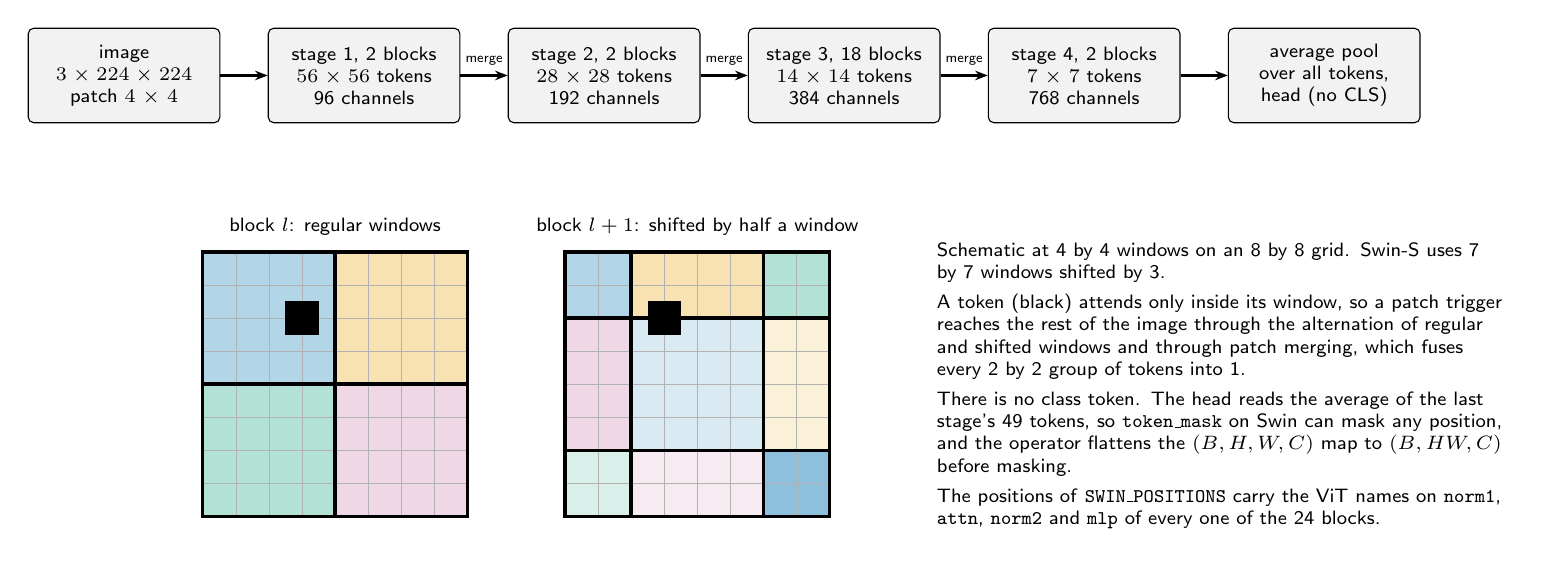
\begin{tikzpicture}

\node[stage] (s0) at (0, 0) {image\\$3\times224\times224$\\patch $4\times4$};
\node[stage, right=6mm of s0] (s1) {stage 1, 2 blocks\\$56\times56$ tokens\\96 channels};
\node[stage, right=6mm of s1] (s2) {stage 2, 2 blocks\\$28\times28$ tokens\\192 channels};
\node[stage, right=6mm of s2] (s3) {stage 3, 18 blocks\\$14\times14$ tokens\\384 channels};
\node[stage, right=6mm of s3] (s4) {stage 4, 2 blocks\\$7\times7$ tokens\\768 channels};
\node[stage, right=6mm of s4] (s5) {average pool\\over all tokens,\\head (no CLS)};
\draw[flow] (s0) -- (s1);
\draw[flow] (s1) -- node[above, font=\tiny\sffamily] {merge} (s2);
\draw[flow] (s2) -- node[above, font=\tiny\sffamily] {merge} (s3);
\draw[flow] (s3) -- node[above, font=\tiny\sffamily] {merge} (s4);
\draw[flow] (s4) -- (s5);

% Regular windows, block l.
\begin{scope}[shift={(1.0,-5.6)}, scale=0.42]
  \fill[w1!30] (0,4) rectangle (4,8);
  \fill[w2!30] (4,4) rectangle (8,8);
  \fill[w3!30] (0,0) rectangle (4,4);
  \fill[w4!30] (4,0) rectangle (8,4);
  \draw[black!30, very thin] (0,0) grid (8,8);
  \draw[very thick] (0,0) rectangle (8,8);
  \draw[very thick] (4,0) -- (4,8);
  \draw[very thick] (0,4) -- (8,4);
  \fill[black] (2.5,5.5) rectangle (3.5,6.5);
  \node[font=\scriptsize\sffamily, anchor=south] at (4,8.2) {block $l$: regular windows};
\end{scope}

% Shifted windows, block l+1: the partition moves by half a window, so tokens
% that sat in different windows now attend to each other.
\begin{scope}[shift={(5.6,-5.6)}, scale=0.42]
  \fill[w1!30] (0,6) rectangle (2,8);
  \fill[w2!30] (2,6) rectangle (6,8);
  \fill[w3!30] (6,6) rectangle (8,8);
  \fill[w4!30] (0,2) rectangle (2,6);
  \fill[w1!15] (2,2) rectangle (6,6);
  \fill[w2!15] (6,2) rectangle (8,6);
  \fill[w3!15] (0,0) rectangle (2,2);
  \fill[w4!15] (2,0) rectangle (6,2);
  \fill[w1!45] (6,0) rectangle (8,2);
  \draw[black!30, very thin] (0,0) grid (8,8);
  \draw[very thick] (0,0) rectangle (8,8);
  \draw[very thick] (2,0) -- (2,8);
  \draw[very thick] (6,0) -- (6,8);
  \draw[very thick] (0,2) -- (8,2);
  \draw[very thick] (0,6) -- (8,6);
  \fill[black] (2.5,5.5) rectangle (3.5,6.5);
  \node[font=\scriptsize\sffamily, anchor=south] at (4,8.2) {block $l+1$: shifted by half a window};
\end{scope}

\node[font=\scriptsize\sffamily, align=left, anchor=north west, text width=72mm]
  at (10.2, -2.0) {%
  Schematic at 4 by 4 windows on an 8 by 8 grid. Swin-S uses 7 by 7 windows shifted
  by 3.\\[3pt]
  A token (black) attends only inside its window, so a patch trigger reaches the rest
  of the image through the alternation of regular and shifted windows and through
  patch merging, which fuses every 2 by 2 group of tokens into 1.\\[3pt]
  There is no class token. The head reads the average of the last stage's 49 tokens,
  so \texttt{token\_mask} on Swin can mask any position, and the operator flattens the
  $(B,H,W,C)$ map to $(B,HW,C)$ before masking.\\[3pt]
  The positions of \texttt{SWIN\_POSITIONS} carry the ViT names on \texttt{norm1},
  \texttt{attn}, \texttt{norm2} and \texttt{mlp} of every one of the 24 blocks.};

\end{tikzpicture}
\end{document}
